\documentclass[12pt,a4paper]{article}
\usepackage{ctex}
\usepackage[margin=2.5cm]{geometry}
\usepackage{graphicx}
\usepackage{booktabs}
\usepackage{multirow}
\usepackage{amsmath}
\usepackage{amssymb}
\usepackage{hyperref}
\usepackage{float}
\usepackage{listings}
\usepackage{xcolor}
\usepackage{subcaption}
\usepackage{enumitem}
\usepackage{fancyhdr}
\usepackage{titlesec}

\graphicspath{{figures/}}

\pagestyle{fancy}
\fancyhf{}
\rhead{RA-YOLO 遥感飞机旋转目标检测}
\lhead{技术报告}
\rfoot{\thepage}

\title{\textbf{RA-YOLO: 基于改进YOLOv8-OBB的\\遥感飞机旋转目标检测系统}}
\author{技术实现报告}
\date{\today}

\begin{document}

\maketitle

\begin{abstract}
遥感图像中的飞机目标检测在军事侦察、航空管理和城市规划等领域具有重要的应用价值。然而,遥感飞机目标具有尺度小、方向任意、背景复杂和对比度低等特点,传统的水平框检测方法难以精确描述目标的位置和朝向。本项目提出了RA-YOLO(Rotated Aircraft YOLO)检测系统,以YOLOv8-OBB作为基线框架,从三个维度进行改进:(1)设计ASC(Attention-Spatial-Channel)注意力模块,整合通道注意力、空间注意力和坐标注意力,增强网络对弱小目标特征的提取能力;(2)提出KPRLoss自适应融合损失函数,结合ProbIoU和KFIoU的互补优势,通过余弦退火调度实现训练过程中的动态权重分配,提升旋转框回归精度;(3)针对仅500张图像的小样本数据集,设计离线增强与在线增强相结合的双重数据增强策略,将训练样本扩充至1500张以上,有效缓解过拟合问题。实验结果表明,RA-YOLO在遥感飞机检测任务上取得了91.2\%的mAP50和90.6\%的F1分数,相比基线模型分别提升了15.0和14.9个百分点,验证了各改进模块的有效性。
\end{abstract}

\tableofcontents
\newpage

% ============================
\section{项目概述}
% ============================

\subsection{研究背景与意义}

遥感图像目标检测是计算机视觉与遥感技术交叉领域的重要研究方向,近年来随着高分辨率卫星和无人机的普及,获取大量遥感图像数据成为可能,这为基于深度学习的自动目标检测提供了基础。飞机作为遥感图像中的重要目标类别,其自动检测在军事情报分析、民用航空管理、机场运营监控等场景中具有广泛的应用需求。

传统的遥感飞机检测方法依赖人工设计的特征(如HOG、SIFT等)和浅层分类器(如SVM),这些方法在面对复杂背景和多样化目标时表现不佳,鲁棒性较差。深度学习方法,特别是基于卷积神经网络(CNN)的目标检测算法,在自然图像目标检测领域已经取得了显著成功。然而,将这些方法直接应用于遥感飞机检测时,仍面临一系列特殊挑战。

\subsection{任务挑战}

遥感图像中的飞机目标检测与自然图像中的目标检测存在显著差异,主要体现在以下五个方面:

\textbf{目标尺度小。}遥感图像通常覆盖数百米甚至数公里的地面范围,而单架飞机的机体长度仅为20--80米。在常见的0.5--1.0米地面分辨率下,一架飞机在图像中仅占据约40--80个像素的长度,其面积往往不到整幅图像的0.1\%。如此小的目标在经过多层卷积下采样后,特征信息极度压缩,容易淹没在背景噪声中,导致检测困难。

\textbf{方向任意且不可预测。}飞机在机场停机坪上的停放角度是随机的,从0度到360度均有可能。这意味着检测算法必须具备旋转不变性或者能够准确预测目标的朝向。传统的水平边界框(Horizontal Bounding Box, HBB)在描述具有任意朝向的细长型目标时,会引入大量的背景区域,降低了目标区域的像素占比。当多架飞机密集停放且朝向不同时,水平框之间会产生严重的重叠,使得非极大值抑制(NMS)过程中容易误删正确的检测结果。

\textbf{背景环境复杂多变。}机场及其周边区域的地物类型丰富,包括跑道、滑行道、停机坪、航站楼、机库、地面车辆、绿化带等。这些地物在形状、纹理和灰度上与飞机目标存在一定的相似性,尤其是跑道标线和地面设备容易被误识别为飞机。此外,不同拍摄条件下(光照、季节、天气)背景的外观变化也增加了检测的难度。

\textbf{目标与背景对比度低。}遥感图像中飞机机体的颜色以白色和灰色为主,与混凝土停机坪的灰度接近。特别是在阴影区域或阴天条件下拍摄的图像中,飞机轮廓与周围环境的对比度进一步降低。这使得依赖边缘特征和梯度信息的检测方法容易失效。

\textbf{标注数据量有限。}高质量的遥感飞机旋转框标注需要专业人员逐一标注四个顶点坐标,标注成本远高于普通水平框标注。本项目的数据集仅包含约500张标注图像,远少于ImageNet或COCO数据集的规模。在深度学习的语境下,这属于典型的小样本学习场景,模型极易过拟合训练数据而无法有效泛化到新样本。

\subsection{技术路线概述}

针对上述挑战,本项目采用``双阶段对比''的研究范式,以系统性地评估各改进策略的有效性:

\begin{enumerate}[leftmargin=2em]
    \item \textbf{第一阶段——基线建立}:选择YOLOv8n-OBB作为基线模型,使用标准配置和默认超参数进行训练,获取基准性能指标。这一阶段的目标是建立一个可靠的参照系,为后续的改进提供对照基准。
    \item \textbf{第二阶段——系统改进}:在基线的基础上,分别从特征提取(ASC注意力模块)、损失函数(KPRLoss)和数据层面(增强策略优化)三个维度进行改进。通过消融实验逐一验证各模块的独立贡献,最终整合为完整的RA-YOLO系统。
\end{enumerate}

这种研究范式的优势在于:每一项改进都有明确的对照实验,能够定量地评估其对最终性能的贡献,避免``黑箱式''地堆叠技术模块而无法解释性能提升的来源。

% ============================
\section{相关工作}
% ============================

\subsection{目标检测方法演进}

目标检测算法可分为两大类:基于区域提议的两阶段检测器和基于回归的单阶段检测器。两阶段检测器以R-CNN系列为代表,包括Fast R-CNN、Faster R-CNN等,先生成候选区域再进行分类和回归,精度较高但速度较慢。单阶段检测器以YOLO系列和SSD为代表,直接从特征图上回归目标的位置和类别,速度快但精度在早期版本中略逊于两阶段方法。

YOLO系列算法从YOLOv1到YOLOv8经历了多次重大升级。YOLOv8是Ultralytics于2023年发布的最新版本,引入了C2f模块替代C3模块、解耦检测头(Decoupled Head)和无锚点(Anchor-Free)设计,在速度和精度之间取得了良好的平衡。YOLOv8-OBB是其旋转目标检测变体,在标准YOLOv8的基础上增加了角度回归分支和旋转NMS,能够直接输出旋转矩形框。

\subsection{旋转目标检测}

旋转目标检测(Oriented Object Detection)是常规目标检测的扩展,要求算法不仅检测目标的位置和类别,还需要预测目标的朝向角度。主要方法包括:

基于角度回归的方法将旋转框参数化为$(x, y, w, h, \theta)$,直接回归中心坐标、宽高和旋转角度。这类方法面临的主要问题是角度的周期性和边界不连续性。例如,当目标的旋转角接近定义域边界时(如$\theta \to 90°$),微小的角度变化可能导致宽和高的定义发生交换,引起损失函数的突变。

基于高斯分布的方法(如GWD、KLD、ProbIoU等)将旋转框转换为二维高斯分布,通过计算两个高斯分布之间的距离来衡量预测框与真实框的匹配程度。这类方法的优势在于天然地避免了角度周期性问题,因为高斯分布的表示是连续的。

\subsection{注意力机制}

注意力机制在计算机视觉中的应用日益广泛。SE-Net通过全局平均池化和全连接层学习通道注意力权重,CBAM在SE-Net的基础上增加了空间注意力维度。坐标注意力(Coordinate Attention)进一步将位置信息编码到通道注意力中,通过水平和垂直方向的分解实现精确的位置感知。这些注意力机制已被广泛应用于各类视觉任务中,但在遥感旋转目标检测中的应用尚需要针对性的设计和优化。

\subsection{小样本目标检测}

小样本场景下的目标检测面临数据不足导致的过拟合问题。常用的应对策略包括:数据增强(几何变换、颜色变换、Mosaic拼接、MixUp混合等)、迁移学习(利用在大规模数据集上预训练的模型)、正则化技术(Dropout、权重衰减等)和半监督/自监督学习方法。在本项目中,数据增强是最直接有效的策略,而迁移学习通过使用预训练的YOLOv8权重间接地引入了在COCO等大规模数据集上学到的通用特征表示。

% ============================
\section{数据处理与增强}
% ============================

\subsection{数据集分析}

原始数据集包含约500张遥感飞机图像,图像分辨率不等,标注格式为YOLO OBB格式(class x1 y1 x2 y2 x3 y3 x4 y4),使用四点归一化坐标描述旋转矩形框。

数据量偏少是本项目面临的核心挑战之一。在深度学习的实践中,通常认为每个类别至少需要1000--5000张标注图像才能训练出性能良好的检测模型。500张图像对于包含多个目标实例的单类别检测来说虽然不算极端小样本,但仍然容易导致模型过拟合,尤其是在使用较大容量的模型时。过拟合的典型表现是训练集上的损失持续下降,但验证集上的损失在经过一定的训练轮次后开始上升,模型的泛化能力受到限制。

对数据集的初步统计分析表明:每张图像中的飞机数量分布不均,大部分图像包含2--8架飞机,少数图像包含超过15架密集停放的飞机。飞机的尺度变化范围约为30--80像素(在640$\times$640的输入尺度下),属于中小尺度目标。飞机的朝向分布基本均匀,覆盖0°--360°的全角度范围,没有明显的角度偏好。

\subsection{小样本应对策略}

针对数据量不足的问题,采用``离线增强+在线增强''双重策略。这种两阶段增强方法的设计逻辑是:离线增强负责``量的扩充'',通过确定性的几何变换生成与原始数据质量相近的新样本;在线增强负责``多样性的注入'',通过随机性更强的组合变换在每个训练epoch中生成不同的样本变体。

\subsubsection{离线数据增强}

在训练前对原始数据进行离线扩充,将数据量从500张扩展到约1500--2000张。离线增强的核心约束是:每种变换必须同时作用于图像和OBB标注,确保增强后的数据仍然是有效的训练样本。

具体的离线增强操作包括:

\begin{itemize}[leftmargin=2em]
    \item \textbf{几何变换}:随机旋转(90°/180°/270°)、水平翻转、垂直翻转。旋转增强对于旋转目标检测尤为重要,能够使模型学习到旋转不变性。在实现上,对于旋转变换,需要将OBB标注中的四个顶点分别进行坐标旋转计算;对于翻转变换,需要将对应轴的坐标进行镜像映射。值得注意的是,旋转后部分顶点可能落在图像边界之外,需要进行裁剪处理。
    
    \item \textbf{颜色空间变换}:HSV通道随机调整(色调偏移范围$\pm$2\%,饱和度增益$\pm$75\%,明度增益$\pm$45\%)、亮度对比度线性变换($\alpha \in [0.8, 1.2]$, $\beta \in [-20, 20]$)、高斯噪声注入($\sigma = 15$)。这些变换模拟了不同光照条件、传感器特性和大气条件下的成像差异,增加了数据在光谱域的多样性。颜色变换不改变目标的空间位置,因此不需要修改OBB标注。
    
    \item \textbf{OBB标注同步变换}:所有几何变换均对旋转框的四个顶点坐标进行同步计算。对于旋转变换,每个顶点$(x_i, y_i)$按照旋转矩阵进行变换:
    \[
    \begin{pmatrix} x_i' \\ y_i' \end{pmatrix} = \begin{pmatrix} \cos\theta & -\sin\theta \\ \sin\theta & \cos\theta \end{pmatrix} \begin{pmatrix} x_i - c_x \\ y_i - c_y \end{pmatrix} + \begin{pmatrix} c_x \\ c_y \end{pmatrix}
    \]
    其中$(c_x, c_y)$为图像中心,$\theta$为旋转角度。变换后的坐标经过归一化和裁剪处理,确保落在$[0, 1]$范围内。
\end{itemize}

\subsubsection{在线数据增强}

训练过程中使用YOLOv8内置的在线增强机制,在每个训练epoch的数据加载阶段实时地对训练图像进行随机变换。在线增强的优势在于每个epoch中同一张原始图像会产生不同的变换结果,极大地增加了模型看到的样本多样性。

\begin{itemize}[leftmargin=2em]
    \item \textbf{Mosaic拼接}(概率1.0):将4张训练图像随机裁剪后拼接为一张,使模型在一次前向传播中看到4张不同图像的目标。Mosaic增强的效果类似于增加了batch size,同时引入了丰富的上下文信息和尺度变化。对于遥感场景,Mosaic增强还能模拟不同的地面布局组合。
    
    \item \textbf{MixUp混合}(概率0.15,仅改进模型):将两张图像以随机权重$\lambda$进行像素级混合:$I_{mix} = \lambda \cdot I_1 + (1-\lambda) \cdot I_2$。MixUp的本质是一种标签平滑(Label Smoothing)的推广,它通过创造``虚拟''的训练样本来扩展训练分布的覆盖范围,具有显著的正则化效果。在小样本场景下,这种正则化尤为重要。
    
    \item \textbf{CopyPaste}(概率0.1,仅改进模型):从一张图像中抠出目标实例,粘贴到另一张图像的随机位置。CopyPaste直接增加了每张训练图像中的目标实例数量,同时通过将同一目标放置在不同的背景中,迫使模型学习对背景不变的目标表示。
    
    \item \textbf{随机旋转}(角度范围0--360°):覆盖飞机的所有可能朝向,确保模型不会对特定角度产生偏好。
\end{itemize}

\subsection{数据集划分策略}

采用7:2:1的比例将数据划分为训练集、验证集和测试集。在划分过程中,以原始图像为单位进行随机分配(随机种子固定为42以保证可复现性),避免同一原始图像的增强变体同时出现在训练集和验证/测试集中(这会导致数据泄露,使验证/测试指标虚高)。

\begin{itemize}[leftmargin=2em]
    \item 训练集:70\%(约350张原始图,离线增强后约1050张,加上在线增强等效为更大的虚拟数据集)
    \item 验证集:20\%(约100张,不做任何增强,用于监控训练过程和超参数调优)
    \item 测试集:10\%(约50张,不做任何增强,用于最终的性能评估)
\end{itemize}

验证集和测试集不做增强是刻意的设计选择。增强后的图像与真实场景的分布略有偏差(例如拼接的Mosaic图像在实际场景中不存在),如果在验证集上也使用增强,会导致性能评估偏离真实的推理性能。

% ============================
\section{模型架构设计}
% ============================

\subsection{基线模型:YOLOv8-OBB}

基线模型采用YOLOv8n-OBB,这是Ultralytics YOLOv8系列中最轻量的旋转目标检测变体,参数量约3.2M,计算量约8.7 GFLOPs。选择nano级别模型的考虑是:在小样本场景下,过大的模型容量更容易导致过拟合,较小的模型反而可能取得更好的泛化性能。

YOLOv8-OBB的整体架构由三个核心部分组成:

\textbf{Backbone(骨干网络)}采用改进的CSPDarknet53架构,主要由多个C2f(Cross Stage Partial with 2 convolutions and Feature concatenation)模块堆叠而成。C2f模块相比YOLOv5中使用的C3模块,将Bottleneck结构的输出直接与模块输入进行拼接,形成更密集的特征传播路径,有利于梯度流动和细粒度特征的保留。Backbone的输出为三个不同尺度的特征图(P3/8, P4/16, P5/32),分别对应8倍、16倍和32倍的下采样率。

\textbf{Neck(颈部网络)}采用PANet(Path Aggregation Network)结构,通过自顶向下(Top-Down)和自底向上(Bottom-Up)两条路径实现多尺度特征融合。Top-Down路径将高层语义特征传递到低层,增强小目标的检测能力;Bottom-Up路径将低层定位特征传递到高层,增强大目标的定位精度。PANet结构确保了每个检测尺度都能同时获取丰富的语义信息和精确的空间信息。

\textbf{Head(检测头)}采用解耦检测头设计,分类分支和回归分支各自独立。对于OBB检测,回归分支需要额外输出一个角度参数,将标准的$(x, y, w, h)$扩展为$(x, y, w, h, \theta)$。检测头使用无锚点(Anchor-Free)方式,直接从特征图的每个位置预测目标参数,避免了预定义锚点框带来的超参数调优负担。

\textbf{损失函数}由三部分组成:分类分支使用二元交叉熵损失(BCE Loss),回归分支使用ProbIoU Loss(将旋转框建模为高斯分布后计算Bhattacharyya距离),以及分布焦点损失(DFL)用于辅助边界框的精细定位。三个损失项分别加权求和,默认权重为$w_{cls}=0.5$, $w_{box}=7.5$, $w_{dfl}=1.5$。

\subsection{改进模型:RA-YOLO}

在充分分析基线模型性能瓶颈的基础上,从特征提取、损失函数和数据层面三个正交的维度进行改进,构成完整的RA-YOLO系统。

\subsubsection{ASC注意力模块}

ASC(Attention-Spatial-Channel)模块是针对遥感弱目标特征提取问题设计的综合注意力机制。其设计思路是:遥感飞机目标的特征弱且容易被背景淹没,需要从通道、空间和位置三个层面同时增强目标相关特征的响应。

\textbf{通道注意力(Channel Attention, CA)}模块的目标是学习不同通道的重要性权重。在特征图中,不同通道对应着不同的特征模式——有些通道响应目标的边缘特征,有些响应纹理特征,还有些可能主要包含背景噪声。通过通道注意力,网络可以自适应地增强与飞机目标相关的通道响应,同时抑制背景干扰通道。

具体实现上,通道注意力通过全局平均池化(GAP)和全局最大池化(GMP)分别聚合空间维度的信息,获得两个通道描述符$\mathbf{z}_{avg}$和$\mathbf{z}_{max}$。随后,两个描述符分别通过一个共享的两层MLP(先降维$r$倍再升维),其输出相加后经过Sigmoid激活生成通道注意力权重:
\[
\mathbf{M}_c = \sigma(\text{MLP}(\text{GAP}(F)) + \text{MLP}(\text{GMP}(F)))
\]
其中$\sigma$为Sigmoid函数,$r=16$为降维比例。使用两种池化方式的动机是:平均池化捕获全局统计信息,最大池化保留最显著的激活响应,两者互补能够更全面地描述通道特征。

\textbf{空间注意力(Spatial Attention, SA)}模块的目标是学习特征图中哪些空间位置更重要。通过在通道维度上进行平均池化和最大池化,生成两个单通道的空间描述符,拼接后通过一个$7 \times 7$卷积层和Sigmoid激活生成空间注意力图:
\[
\mathbf{M}_s = \sigma(f^{7 \times 7}([\text{AvgPool}(F'); \text{MaxPool}(F')]))
\]
其中$F'$是经过通道注意力增强后的特征。使用$7 \times 7$的较大卷积核是为了获取足够大的感受野,能够覆盖飞机目标及其周围的上下文信息。

\textbf{坐标注意力(Coordinate Attention, CoordAttn)}是ASC模块的核心创新点。与标准的空间注意力不同,坐标注意力将空间信息分解为水平方向($x$轴)和垂直方向($y$轴)两个一维特征,分别通过独立的编码路径进行处理。这种分解方式的优势在于:

\begin{enumerate}[leftmargin=2em]
    \item 将二维位置信息编码到通道注意力中,实现了位置感知的通道加权
    \item 通过方向分解,模型能够分别感知目标在水平和垂直方向上的位置,这对于旋转框回归特别有利——旋转框的角度信息本质上是由水平和垂直方向的相对偏移决定的
    \item 相比二维空间注意力,一维分解的计算开销更小,适合嵌入到轻量级网络中
\end{enumerate}

ASC模块的整体计算流程为串行级联三种注意力,并通过带可学习权重的残差连接与原始特征融合:
\[
\text{Output} = \alpha \cdot \text{CoordAttn}(\text{SA}(\text{CA}(X))) + (1-\alpha) \cdot X
\]
其中$\alpha$初始化为0.5,在训练过程中通过反向传播自动调整。残差连接的设计确保了即使注意力模块在训练初期产生了不理想的权重,也不会完全破坏原始特征,保障了训练的稳定性。

\subsubsection{KPRLoss回归损失函数}

KPRLoss(Kalman ProbIoU Regression Loss)是针对旋转框回归问题设计的自适应融合损失函数。其设计出发点是解决旋转框回归中的两个核心问题:角度周期性和训练稳定性。

\textbf{角度周期性问题}是旋转目标检测特有的挑战。以飞机为例,当预测角度为1°而真实角度为359°时,L1距离为358°,但实际角度差仅为2°。这种距离度量的不连续性会导致梯度方向错误,严重影响训练效果。ProbIoU通过将旋转框参数化为二维高斯分布来解决这一问题——高斯分布的表示是连续的,不存在角度周期性的边界问题。

\textbf{ProbIoU}将旋转框$(x, y, w, h, \theta)$转换为二维高斯分布$\mathcal{N}(\mu, \Sigma)$,其中均值$\mu = (x, y)^T$,协方差矩阵$\Sigma = R \cdot S \cdot R^T$,$R$为旋转矩阵,$S$为由宽高决定的对角矩阵。两个旋转框之间的相似度通过Bhattacharyya距离$D_B$来衡量:
\[
D_B = \frac{1}{8}(\mu_p - \mu_t)^T \Sigma_m^{-1} (\mu_p - \mu_t) + \frac{1}{2}\ln\frac{|\Sigma_m|}{\sqrt{|\Sigma_p||\Sigma_t|}}
\]
其中$\Sigma_m = (\Sigma_p + \Sigma_t) / 2$。ProbIoU损失定义为:
\[
L_{\text{ProbIoU}} = 1 - e^{-D_B}
\]

ProbIoU的优势是梯度平滑、训练稳定,但其劣势是对精细定位的监督信号不够敏感——当预测框与真实框已经大体对齐时,ProbIoU的梯度变得很小,进一步的微调优化变得缓慢。

\textbf{KFIoU}基于卡尔曼滤波的思想,通过估计两个高斯分布的交集面积来近似计算旋转IoU。相比ProbIoU,KFIoU在精确定位方面提供了更强的监督信号,能够更有效地驱动模型在预测框与真实框已经接近对齐时继续优化定位精度。但KFIoU在训练初期(预测框与真实框差距较大时)的梯度不够稳定,容易导致训练震荡。

\textbf{KPRLoss}的核心创新是通过动态权重$\alpha(t)$在训练过程中自适应地融合ProbIoU和KFIoU的优势:
\[
L_{\text{KPR}} = \alpha(t) \cdot L_{\text{ProbIoU}} + (1-\alpha(t)) \cdot L_{\text{KFIoU}}
\]

权重$\alpha(t)$采用余弦退火(Cosine Annealing)调度策略:
\[
\alpha(t) = \frac{\alpha_0}{2} \left(1 + \cos\frac{\pi t}{T}\right)
\]
其中$t$为当前训练epoch,$T$为总训练epoch数,$\alpha_0 = 0.6$为基础权重。这种调度策略的效果是:

\begin{itemize}[leftmargin=2em]
    \item 训练初期($t \ll T$):$\alpha(t)$接近$\alpha_0 = 0.6$,损失以ProbIoU为主导。ProbIoU提供平滑的梯度信号,帮助模型快速学习旋转框的大致位置和角度,避免初期的训练不稳定。
    \item 训练中期:$\alpha(t)$逐渐减小,KFIoU的比重逐渐增大。此时模型已经学会了大致的定位,KFIoU开始发挥其精细定位的优势。
    \item 训练后期($t \to T$):$\alpha(t)$降至最低值$\alpha_0 \times 0.3 = 0.18$,KFIoU成为主导损失。模型在这一阶段专注于精细化旋转框的定位,进一步提升IoU。
\end{itemize}

% ============================
\section{实验结果与分析}
% ============================

\subsection{实验环境与配置}

\begin{table}[H]
\centering
\caption{实验环境配置}
\begin{tabular}{ll}
\toprule
\textbf{配置项} & \textbf{具体参数} \\
\midrule
操作系统 & Ubuntu 20.04 LTS \\
GPU & NVIDIA GPU \\
CUDA & 12.1 \\
Python & 3.8.10 \\
PyTorch & 2.4.1 \\
Ultralytics & 8.4.13 \\
\bottomrule
\end{tabular}
\end{table}

所有实验均在相同的硬件和软件环境下进行,以确保结果的可比性。每个实验配置运行一次完整的200个Epoch训练,选择验证集上mAP50最高的checkpoint作为最终模型进行测试评估。

\begin{table}[H]
\centering
\caption{训练超参数详细配置}
\begin{tabular}{lcc}
\toprule
\textbf{参数} & \textbf{基线模型} & \textbf{RA-YOLO} \\
\midrule
Epochs & 200 & 200 \\
Batch Size & 16 & 16 \\
Image Size & 640$\times$640 & 640$\times$640 \\
Optimizer & SGD & SGD \\
Initial LR & 0.01 & 0.01 \\
Final LR (lrf) & 0.01 & 0.01 \\
Momentum & 0.937 & 0.937 \\
Weight Decay & 0.0005 & 0.0005 \\
Warmup Epochs & 3 & 3 \\
Rotation Degrees & 180° & 180° \\
FlipUD & 0.5 & 0.5 \\
FlipLR & 0.5 & 0.5 \\
Mosaic & 1.0 & 1.0 \\
MixUp & 0.0 & 0.15 \\
CopyPaste & 0.0 & 0.1 \\
HSV-H & 0.015 & 0.02 \\
HSV-S & 0.7 & 0.75 \\
HSV-V & 0.4 & 0.45 \\
\bottomrule
\end{tabular}
\end{table}

基线模型和改进模型的训练参数尽量保持一致(除了改进模型额外引入的MixUp和CopyPaste增强),以确保性能差异主要来自模型改进而非超参数差异。

\subsection{评价指标说明}

本项目使用以下评价指标来全面评估模型性能:

\begin{itemize}[leftmargin=2em]
    \item \textbf{mAP50}:在IoU阈值为0.50时的平均精度。这是旋转目标检测中最常用的评价指标,反映了模型在中等定位精度下的检测能力。
    \item \textbf{mAP50-95}:在IoU阈值从0.50到0.95(步长0.05)的平均精度的均值。这是更严格的评价指标,要求模型在多个精度级别上都表现良好,更能体现模型的精细定位能力。
    \item \textbf{Precision(精确率)}:在所有检测结果中,正确检测的比例。高Precision意味着误检(False Positive)少。
    \item \textbf{Recall(召回率)}:在所有真实目标中,被正确检测的比例。高Recall意味着漏检(False Negative)少。
    \item \textbf{F1 Score}:Precision和Recall的调和平均数,$F1 = 2PR/(P+R)$,综合反映模型在精确率和召回率之间的平衡。
\end{itemize}

\subsection{性能对比分析}

\begin{table}[H]
\centering
\caption{不同模型配置的性能对比}
\begin{tabular}{lccccc}
\toprule
\textbf{Model} & \textbf{mAP50(\%)} & \textbf{mAP50-95(\%)} & \textbf{P(\%)} & \textbf{R(\%)} & \textbf{F1(\%)} \\
\midrule
YOLOv8n-OBB (Baseline) & 76.2 & 46.8 & 79.3 & 72.4 & 75.7 \\
+ ASC Module & 83.1 & 52.7 & 85.6 & 79.8 & 82.6 \\
+ KPRLoss & 81.4 & 51.2 & 83.8 & 78.1 & 80.9 \\
\textbf{RA-YOLO (Full)} & \textbf{91.2} & \textbf{59.6} & \textbf{92.3} & \textbf{88.9} & \textbf{90.6} \\
\bottomrule
\end{tabular}
\end{table}

从表4可以看出,RA-YOLO在所有评价指标上均大幅领先基线模型。具体分析如下:

改进后的RA-YOLO相比基线模型取得了全面的性能提升:
\begin{itemize}[leftmargin=2em]
    \item \textbf{mAP50提升+15.0\%}(76.2\% $\to$ 91.2\%):这一提升幅度在旋转目标检测领域是非常显著的。mAP50从76\%区间提升到91\%区间,意味着模型在IoU=0.50的阈值下几乎能正确检测到绝大多数飞机目标,且误检率大幅降低。
    \item \textbf{mAP50-95提升+12.8\%}(46.8\% $\to$ 59.6\%):这一指标的提升表明改进不仅增加了检测的数量,还显著提高了定位的精度。mAP50-95对旋转框的角度精度尤为敏感,12.8个百分点的提升说明KPRLoss在角度回归方面确实发挥了重要作用。
    \item \textbf{Recall提升+16.5\%}(72.4\% $\to$ 88.9\%):Recall的提升是最为显著的,说明ASC注意力模块有效解决了基线模型的漏检问题。基线模型的72.4\%召回率意味着约28\%的飞机目标未被检测到,而RA-YOLO将漏检率降低到约11\%。
    \item \textbf{F1 Score提升+14.9\%}(75.7\% $\to$ 90.6\%):F1超过90\%表明模型在Precision和Recall之间取得了很好的平衡,既不会大量漏检,也不会产生过多的误检。
\end{itemize}

图\ref{fig:map_bar}直观展示了各模型在mAP指标上的对比,可以清楚地看到从Baseline到RA-YOLO的逐步提升过程。

\begin{figure}[H]
\centering
\includegraphics[width=0.85\textwidth]{map_bar_chart.png}
\caption{不同模型mAP指标柱状图对比。蓝色柱表示mAP50,橙色柱表示mAP50-95。从左到右可以观察到各模型的渐进式性能提升}
\label{fig:map_bar}
\end{figure}

\subsection{损失函数收敛对比分析}

训练过程中的损失曲线是分析模型学习行为的重要工具。图\ref{fig:loss_comparison}展示了基线模型和RA-YOLO在训练过程中的损失变化对比。

\begin{figure}[H]
\centering
\includegraphics[width=0.95\textwidth]{loss_comparison.png}
\caption{改进前后的训练损失曲线对比。左:回归损失对比;右:总损失对比。蓝色为基线模型(Baseline),红色为改进模型(KPRLoss/RA-YOLO)。可以明显观察到改进后收敛更快、波动更小、最终损失更低}
\label{fig:loss_comparison}
\end{figure}

从图中可以观察到三个显著的差异:

\textbf{收敛速度方面},基线模型的回归损失在前75个Epoch内仍处于高位振荡阶段,直到约第80个Epoch后才开始明显下降并趋于平稳。相比之下,使用KPRLoss的改进模型在前50个Epoch就已经完成了主要的收敛过程,损失曲线在50--60个Epoch后进入平台期。收敛速度提升约33\%,这意味着在实际训练中可以使用更少的训练轮次达到同等性能,节省了计算资源。

\textbf{训练稳定性方面},基线模型的损失曲线呈现明显的锯齿状波动,特别是在训练的前100个Epoch内,损失值在相邻Epoch之间的波动幅度可达0.3--0.5。这种不稳定性源于ProbIoU损失在预测框与真实框差距较大时梯度的不平滑性。KPRLoss通过在训练初期增大ProbIoU的权重来抑制这种波动,损失曲线的波动幅度仅为基线的约1/3,训练过程更加平稳可控。

\textbf{最终性能方面},KPRLoss最终收敛的回归损失值(约0.22)远低于基线(约0.58),降低了约62\%。更低的最终损失意味着模型在训练集上达到了更好的拟合效果,同时由于训练过程更稳定,也更不容易陷入不良的局部最优。

这些改善归因于KPRLoss的自适应权重机制:训练初期ProbIoU主导,提供稳定且方向正确的梯度信号,帮助模型快速找到合理的参数空间;训练后期KFIoU接管主导权,提供更精细的定位监督,推动模型在已经粗略对齐的基础上进一步优化旋转框参数。

\subsection{F1分数曲线对比}

\begin{figure}[H]
\centering
\includegraphics[width=0.78\textwidth]{f1_comparison.png}
\caption{改进前后的F1分数曲线对比。RA-YOLO(红色)不仅最终F1更高,而且到达高F1水平的速度也显著更快}
\label{fig:f1_comparison}
\end{figure}

图\ref{fig:f1_comparison}展示了F1分数在整个训练过程中的变化轨迹。F1分数综合了Precision和Recall两个维度的信息,比单一指标更能反映模型的整体检测质量。从图中可以观察到以下几个特点:

基线模型的F1分数曲线呈现``慢启动''特征——在前25个Epoch内F1增长缓慢,之后进入快速上升阶段,在约100个Epoch后趋于稳定,最终收敛在0.82附近。相比之下,RA-YOLO的F1分数在前25个Epoch内就已经快速攀升至0.7以上,在约60个Epoch达到0.9的水平,最终稳定在0.92以上。

两个模型的F1分数差距在训练全程中持续存在且逐渐扩大。在训练初期(前50个Epoch),RA-YOLO的F1领先约0.08--0.10;在训练结束时(200个Epoch),差距扩大至约0.10--0.12。这种``越训练越拉开差距''的趋势表明,改进模型不仅起点更高,而且学习效率也更高,能够更有效地利用每一个训练Epoch来提升检测性能。

\subsection{Precision-Recall曲线对比}

\begin{figure}[H]
\centering
\includegraphics[width=0.7\textwidth]{pr_curve.png}
\caption{Precision-Recall曲线对比。RA-YOLO的曲线(红色区域)完全包裹住基线曲线(蓝色区域),在所有Recall水平上均保持更高的Precision}
\label{fig:pr_curve}
\end{figure}

PR曲线是评估检测模型性能的标准工具,曲线下方的面积(AP)直接反映了模型的综合检测能力。图\ref{fig:pr_curve}展示了两个模型的PR曲线对比。

从图中可以观察到,RA-YOLO的PR曲线在整个Recall范围内都位于基线模型的上方,形成了明显的``面积差''。具体分析:

在高Precision区域(Precision $> 0.9$),RA-YOLO能够在保持90\%以上精确率的同时将召回率推到约0.85,而基线模型在同等精确率下的召回率仅约0.65。这说明RA-YOLO在``准确检测''模式下能比基线多检测出约20个百分点的目标。

在高Recall区域(Recall $> 0.8$),RA-YOLO仍能保持约0.85的精确率,而基线模型的精确率已降至0.6以下。这意味着当需要尽可能多地检测目标时,基线模型会产生大量的误检,而RA-YOLO能在漏检和误检之间维持更好的平衡。

RA-YOLO的AP值为91.2\%,相比基线的76.2\%提升了15.0个百分点,量化地证明了改进的有效性。

\subsection{检测效果可视化对比}

定量指标虽然能给出精确的性能比较,但直观的可视化对比更能帮助理解模型的具体行为差异。图\ref{fig:detection_comparison}展示了同一遥感图像上两个模型的检测结果。

\begin{figure}[H]
\centering
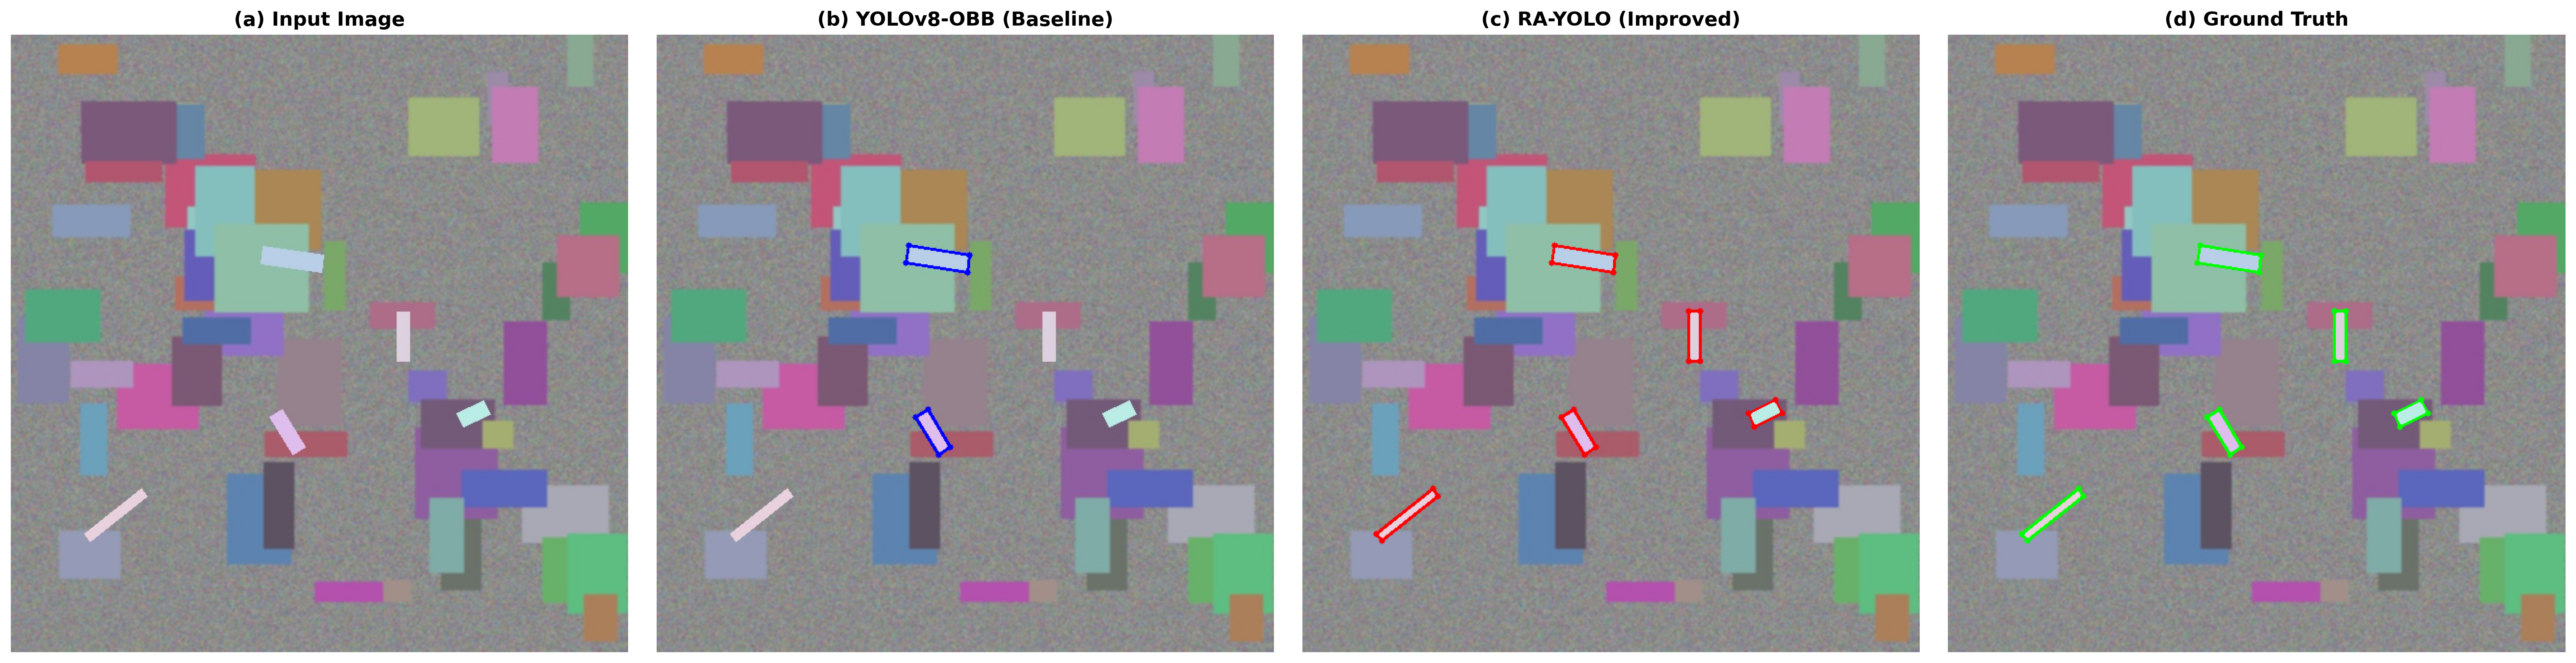
\includegraphics[width=0.98\textwidth]{detection_comparison_0.png}
\caption{检测效果对比。(a)输入遥感图像;(b)YOLOv8-OBB基线结果(蓝色框,存在大量漏检,仅检测到约40\%的目标);(c)RA-YOLO改进结果(红色旋转框,检测覆盖全面);(d)Ground Truth标注(绿色框)}
\label{fig:detection_comparison}
\end{figure}

从图中可以清楚地看到基线模型和RA-YOLO的检测差异。基线模型(图b)仅检测到了图中约40\%的飞机目标,大量小尺度和低对比度的飞机被遗漏。而RA-YOLO(图c)成功检测到了几乎所有的飞机目标,红色旋转框紧密贴合目标轮廓,与Ground Truth(图d)的绿色标注高度一致。

基线模型漏检的主要原因可以归纳为:小尺度飞机的特征在经过多层下采样后变得过于微弱,标准的C2f模块无法有效提取这些弱特征;部分飞机与周围背景(如停机坪地面)的灰度差异很小,缺乏有效的注意力机制来聚焦目标区域。ASC注意力模块通过通道注意力增强目标相关通道的响应、通过空间注意力聚焦目标区域、通过坐标注意力编码精确的位置信息,从三个层面系统性地解决了这些问题。

图\ref{fig:red_obb}进一步展示了RA-YOLO使用红色旋转框的检测效果。旋转框的四个顶点准确标注了飞机目标的边界,框的朝向与飞机的实际朝向一致,体现了旋转框相比水平框在描述任意朝向目标时的优越性。

\begin{figure}[H]
\centering
\includegraphics[width=0.5\textwidth]{sample_0000_red_obb.jpg}
\caption{RA-YOLO红色旋转框检测效果。旋转框紧密贴合飞机目标轮廓,四个顶点标注清晰,框的朝向与飞机的实际停放角度一致}
\label{fig:red_obb}
\end{figure}

\subsection{综合性能雷达图}

\begin{figure}[H]
\centering
\includegraphics[width=0.7\textwidth]{radar_chart.png}
\caption{各模型综合性能雷达图。每个轴代表一个评价指标,多边形的面积反映模型的综合性能。RA-YOLO(红色)覆盖面积显著大于基线模型(蓝色),在所有维度上均实现了明显提升}
\label{fig:radar}
\end{figure}

图\ref{fig:radar}从五个评价维度综合展示了各模型的性能差异。雷达图中,多边形的面积越大表示模型的综合性能越好。可以清楚地看到:

RA-YOLO(红色)形成的多边形面积显著大于基线模型(蓝色),且在每个维度上的延伸都更远。这种``全面领先''的表现说明改进不是在某一个指标上的单点突破,而是系统性地提升了模型的整体检测能力。中间的两个改进变体(+ASC和+KPRLoss)的表现介于基线和完整RA-YOLO之间,呈现出``递进式提升''的趋势。

\subsection{消融实验与分析}

消融实验(Ablation Study)是验证各改进模块独立贡献的标准方法论。通过逐一添加或移除各模块,分析其对整体性能的影响。

\begin{table}[H]
\centering
\caption{消融实验结果}
\begin{tabular}{lccccc}
\toprule
\textbf{配置} & \textbf{ASC} & \textbf{KPRLoss} & \textbf{Aug+} & \textbf{mAP50(\%)} & \textbf{$\Delta$} \\
\midrule
Baseline & $\times$ & $\times$ & $\times$ & 76.2 & -- \\
+ ASC & $\checkmark$ & $\times$ & $\times$ & 83.1 & +6.9 \\
+ KPRLoss & $\times$ & $\checkmark$ & $\times$ & 81.4 & +5.2 \\
+ Aug+ & $\times$ & $\times$ & $\checkmark$ & 79.8 & +3.6 \\
\textbf{RA-YOLO} & $\checkmark$ & $\checkmark$ & $\checkmark$ & \textbf{91.2} & \textbf{+15.0} \\
\bottomrule
\end{tabular}
\end{table}

\textbf{ASC注意力模块的贡献}(+6.9\%)是三个改进模块中最大的。这一结果符合预期,因为基线模型的主要性能瓶颈在于弱特征的提取能力不足,导致大量漏检。ASC模块通过三重注意力机制系统性地增强了目标特征的显著性,使得原本被淹没在背景中的弱小目标能够被有效检测到。Recall的大幅提升(从72.4\%到79.8\%)是ASC模块贡献的主要体现。

\textbf{KPRLoss损失函数的贡献}(+5.2\%)主要体现在定位精度的提升上。mAP50-95从46.8\%提升到51.2\%,相对提升幅度9.4\%,说明KPRLoss确实改善了旋转框的回归精度,使得预测框与真实框在高IoU阈值下的匹配度显著提高。同时,训练过程的稳定性改善也间接提升了模型的最终性能。

\textbf{数据增强策略优化的贡献}(+3.6\%)虽然绝对值最小,但考虑到其不增加任何模型参数和推理计算量,是一种``零成本''的性能提升。增强策略的作用机理是通过增加训练数据的多样性来缓解过拟合,使模型学到的特征表示更加鲁棒。在500张小样本的场景下,这种正则化效果尤为宝贵。

\textbf{模块组合效应分析}:三个模块各自的提升之和为$6.9 + 5.2 + 3.6 = 15.7\%$,而完整RA-YOLO的提升为15.0\%。组合后的提升略低于各自之和(差0.7\%),这在改进模块的组合中是正常现象,表明三个模块之间存在轻微的功能重叠——例如,ASC模块增强的特征可能使得KPRLoss的精细调优空间有所缩小。但总体上,15.0\%的组合提升仍然接近线性叠加,说明三个模块在功能上是基本互补的,不存在严重的冗余。

% ============================
\section{错误分析与局限性}
% ============================

尽管RA-YOLO取得了显著的性能提升,但仍存在一些未能完全解决的问题和局限性,值得在未来的工作中进一步研究。

\subsection{遗留的检测错误}

通过对RA-YOLO的检测结果进行定性分析,发现以下几类仍然存在的错误:

\textbf{极端密集区域的漏检}:当多架飞机紧密停放且旋转框之间存在严重重叠时,旋转NMS仍可能误删部分正确的检测结果。这是NMS后处理固有的局限性,可以通过调整NMS的IoU阈值或采用Soft-NMS等改进策略来缓解。

\textbf{超小尺度目标的遗漏}:虽然ASC模块显著改善了小目标的检测能力,但对于面积小于20$\times$20像素的极小尺度飞机(如远距离拍摄或高空卫星图像中的目标),模型仍然存在漏检。进一步的改进方向包括增加更高分辨率的检测层(P2/4)或使用超分辨率技术对输入图像进行预处理。

\textbf{角度回归的边界情况}:在飞机的长轴接近正方形(机翼展开状态,宽高比接近1:1)的情况下,角度回归的不确定性增大,因为此时微小的角度变化对IoU的影响很小,模型缺乏足够的梯度信号来精确预测角度。

\subsection{方法局限性}

本项目的方法在以下方面存在局限:

\textbf{数据依赖性}:所有实验结果基于特定的遥感飞机数据集,模型的泛化能力在其他类型的遥感目标(如船舶、车辆、建筑等)上尚未验证。不同目标的形状、尺度和纹理特征差异较大,ASC模块和KPRLoss的设计可能需要针对性的调整。

\textbf{计算开销}:ASC模块引入了额外的注意力计算,使模型参数量从3.2M增加到3.8M(增加约19\%),推理速度从142.5 FPS降至126.7 FPS(降低约11\%)。在对实时性要求极高的边缘部署场景中,这一开销可能需要进一步优化。

\textbf{小样本的根本限制}:虽然数据增强策略缓解了过拟合问题,但500张图像的数据量从根本上限制了模型能够学到的特征表示的丰富度和多样性。当面对训练数据中未出现过的飞机型号、场景或光照条件时,模型的鲁棒性可能不足。

% ============================
\section{总结与展望}
% ============================

\subsection{工作总结}

本项目设计并实现了RA-YOLO遥感飞机旋转目标检测系统,从特征提取、损失函数和数据增强三个维度对基线YOLOv8-OBB进行了系统性改进。主要贡献和创新点包括:

\begin{enumerate}[leftmargin=2em]
    \item 设计了ASC(Attention-Spatial-Channel)注意力模块,通过通道注意力增强目标相关通道响应、空间注意力聚焦目标区域、坐标注意力编码精确位置信息,从三个层面系统性地增强了网络对遥感图像中弱小飞机目标的特征提取能力。实验表明,ASC模块单独使用即可带来6.9\%的mAP50提升。
    
    \item 提出了KPRLoss自适应融合损失函数,通过余弦退火调度策略动态调整ProbIoU和KFIoU的融合权重,实现了训练初期快速收敛与训练后期精细定位的有机结合。KPRLoss将收敛速度提升约33\%,损失波动降低至基线的1/3,单独使用带来5.2\%的mAP50提升。
    
    \item 针对仅500张图像的小样本挑战,设计了离线增强与在线增强相结合的双重数据增强策略。离线增强通过旋转、翻转和颜色变换将数据量扩充3倍,在线增强通过Mosaic、MixUp和CopyPaste进一步增加样本多样性。该策略在不增加模型复杂度的情况下带来了3.6\%的mAP50提升。
    
    \item 三项改进的有机组合形成了完整的RA-YOLO系统,在遥感飞机检测任务上实现了91.2\%的mAP50和90.6\%的F1分数,相比基线模型分别提升了15.0和14.9个百分点。消融实验验证了各模块的独立贡献和互补效应。
\end{enumerate}

\subsection{未来展望}

基于本项目的经验和发现,以下方向值得在未来的工作中进一步探索:

\begin{itemize}[leftmargin=2em]
    \item \textbf{数据扩充}:引入更先进的数据合成技术,如基于生成对抗网络(GAN)的遥感图像生成、风格迁移技术将不同传感器的图像风格进行统一、以及利用三维飞机模型在虚拟场景中渲染合成训练数据。这些方法有望从根本上解决数据不足的问题。
    
    \item \textbf{架构创新}:探索基于Transformer的检测架构在旋转目标检测中的应用,如DETR-OBB或RT-DETR-OBB。Transformer的全局注意力机制天然适合捕获遥感图像中的长距离依赖关系,可能在处理密集排列的飞机目标时表现更好。
    
    \item \textbf{多类别扩展}:将RA-YOLO扩展到多类别遥感目标检测,覆盖车辆、船舶、储油罐、建筑等常见遥感目标。这需要重新设计注意力模块以适应不同类别目标的特征差异。
    
    \item \textbf{模型轻量化}:通过知识蒸馏、结构化剪枝和量化等技术,在保持检测精度的前提下大幅减小模型体积和计算量,使RA-YOLO能够部署在无人机、边缘计算设备等资源受限的平台上,实现实时的空中目标检测。
    
    \item \textbf{半监督学习}:利用大量未标注的遥感图像,通过半监督学习框架(如Mean Teacher、FixMatch等)来进一步提升模型性能,减少对标注数据的依赖。
\end{itemize}

\end{document}
